% !TEX root = task-1-11-1.tex
% Editable task bank. Append new BankTask blocks at the end of the document.
\documentclass[12pt,a4paper]{article}
\usepackage{physics-textbook}
\usepackage{graphicx,needspace}
\usetikzlibrary{decorations.pathmorphing}
\newif\ifShowSolutions
\ifdefined\TutorEdition
  \ShowSolutionstrue
\else
  \ShowSolutionsfalse % Change to \ShowSolutionstrue to display solutions.
\fi
\newcounter{banktask}
\newsavebox{\BankTaskBox}
\newcommand{\BankTaskContent}[3]{%
  \noindent\textbf{\thebanktask.}\quad #2\par
  \ifShowSolutions
    \Needspace{50mm}% Keep the solution heading with its opening text or diagram.
    #3\par
    \ifdefined\TutorEdition
      \ifcsname TutorSource#1\endcsname
        \nopagebreak\smallskip{\small\csname TutorSource#1\endcsname\par}%
      \fi
    \fi
  \fi
}
\newcommand{\BankTask}[3]{%
  \refstepcounter{banktask}\par\medskip
  \sbox{\BankTaskBox}{\begin{minipage}{\linewidth}%
    \BankTaskContent{#1}{#2}{#3}\end{minipage}}%
  \ifdim\dimexpr\ht\BankTaskBox+\dp\BankTaskBox\relax>\dimexpr\textheight-20mm\relax
    \Needspace{35mm}\BankTaskContent{#1}{#2}{#3}%
  \else
    \Needspace{\dimexpr\ht\BankTaskBox+\dp\BankTaskBox\relax}%
    \noindent\usebox{\BankTaskBox}\par
  \fi
  \medskip
}
\begin{document}
\BookSubsection{1.11.1}{Сухое трение}


% Source sdamgia-334: https://phys-ege.sdamgia.ru/problem?id=334
\BankTask{sdamgia-334}{
Тело равномерно движется по плоскости. Сила давления тела на плоскость равна $20\,\text{Н}$, сила трения $5\,\text{Н}$. Чему равен коэффициент трения скольжения?
}{
\smallskip\noindent\textbf{Решение}\par
Сила давления на плоскость, сила трения и коэффициент трения связаны соотношением $F_=\mu P.$ Следовательно, коэффициент трения равен: 

\[\mu = \frac{F_{\text{тр}}}{P} = \frac{5\,\text{Н}}{20\,\text{Н}} =0{,}25.\]

Ответ: $0{,}25$.
}

% Source sdamgia-732: https://phys-ege.sdamgia.ru/problem?id=732
\BankTask{sdamgia-732}{
На горизонтальном полу стоит ящик массой $10\,\text{кг}$. Коэффициент трения между полом и ящиком равен $0{,}25$. К ящику в горизонтальном направлении прикладывают силу $16\,\text{Н}$. Какова сила трения между ящиком и полом? Ответ выразите в ньютонах.
}{
\smallskip\noindent\textbf{Решение}\par
Определим, какую величину имеет сила трения скольжения:

\[F_{\text{тр. скол.}}=\mu N=\mu mg=0{,}25 \cdot  10\,\text{кг} \cdot  10\,\text{м/с} ^2 =25\,\text{Н}.\]

Поскольку сила трения скольжения превосходит по величине силу $F=16\,\text{Н},$ с которой ящик толкают в горизонтальном направлении, ящик останется стоять на месте. Следовательно, согласно второму закону Ньютона, сила трения между ящиком и полом будет равняться по модулю силе $F.$

Ответ: $16$.
}

% Source sdamgia-3547: https://phys-ege.sdamgia.ru/problem?id=3547
\BankTask{sdamgia-3547}{
Два спортсмена разной массы на одинаковых автомобилях, движущихся со скоростью $v _1 = 10\,\text{км/ч}$ и $v _2 = 20\,\text{км/ч},$ стали тормозить, заблокировав колеса. Каково отношение $s_1/s_2$ тормозных путей их автомобилей при одинаковом коэффициенте трения колес о землю?
}{
\smallskip\noindent\textbf{Решение}\par
При торможении на автомобили действует сила трения скольжения, которая и останавливает их. Величина силы трения скольжения определяется выражением $F_{\text{тр}}=\mu N,$ где $N$ — сила реакции опоры, которую можно найти, выписав второй закон Ньютона в проекции на вертикальную ось: $N - mg =0 \Longleftrightarrow  N=mg.$

Вычислим теперь ускорение, с которым тормозит каждый из спортсменов. Второй закон Ньютона в проекции на горизонтальную ось дает $F_{\text{тр}}=\mu mg=ma \Longleftrightarrow  a=\mu g$ (здесь $m$ — масса автомобиля вместе со спортсменом). Поскольку ускорение не зависит от массы, заключаем, что оба автомобиля тормозят с одинаковым ускорением.

Тормозной путь можно найти по формуле $S= \frac{v _0 ^2}{2a} ,$ где $v _0$ — начальная скорость. Следовательно, отношение тормозных путей равно:

\[\frac{s_1}{s_2} = \frac{v _{01} ^2 /2a}{v _{02} ^2 /2a} = \frac{v _{01} ^2}{v _{02} ^2} = \frac{( 10\,\text{км/ч} ) ^2}{( 20\,\text{км/ч} ) ^2} = \frac{1}{4} =0{,}25.\]

Ответ: $0{,}25$.
}

% Source sdamgia-10632: https://phys-ege.sdamgia.ru/problem?id=10632
\BankTask{sdamgia-10632}{
Небольшое тело кладут на наклонную плоскость, угол при основании которой можно изменять. Если угол при основании наклонной плоскости равен $20^\circ$, то тело покоится и на него действует такая же по модулю сила трения, как и в случае, когда угол при основании наклонной плоскости равен $47^\circ$. Чему равен коэффициент трения между наклонной плоскостью и телом? Ответ округлите до десятых долей.
}{
\smallskip\noindent\textbf{Решение}\par
Запишем второй закон Ньютона в первом случае, когда тело покоится:

\[\vec F_{\text{тр}} + \vec N + m\vec g=0.\]

В проекции на ось, параллельную наклонной плоскости:

\[F_{\text{тр}}1=mg \sin  \alpha  _1.\]

Если бы во втором случае тело тоже покоилось, то сила трения была бы $mg \sin  \alpha  _2$ и не могла бы равняться $F_{\text{тр}}1.$ Значит, при угле $47^\circ$ тело скользит. Запишем второй закон Ньютона во втором случае в проекции на ось, перпендикулярную плоскости:

\[N=mg \cos  \alpha  _2.\]

Сила трения скольжения равна:

\[F_{\text{тр}}2=\mu N = \mu mg \cos  \alpha  _2,\]

Приравнивая силы, получаем:

\[F_{\text{тр}}1= F_{\text{тр}}2 \Longleftrightarrow  mg \sin  \alpha  _1 = \mu mg \cos  \alpha  _2.\]

Выразим отсюда коэффициент трения между наклонной плоскостью и телом:

\[\mu = \frac{\sin  \alpha  _1}{\cos  \alpha  _2} = \frac{\sin  20 ^\circ}{\cos  47 ^\circ} \approx 0{,}5.\]

Ответ: $0{,}5$.
}

% Source sdamgia-16847: https://phys-ege.sdamgia.ru/problem?id=16847
\BankTask{sdamgia-16847}{
На шероховатой наклонной плоскости покоится деревянный брусок. Угол наклона плоскости увеличили, но брусок относительно плоскости остался в покое. Как изменились при этом сила нормального давления бруска на плоскость и коэффициент трения бруска о плоскость?

Для каждой величины определите соответствующий характер изменения.

$1$. Увеличилась.

$2$. Уменьшилась.

$3$. Не изменилась.

 

\begin{center}\small\renewcommand{\arraystretch}{1.25}\begin{tabular}{|p{0.450\linewidth}|p{0.450\linewidth}|}\hline
Сила нормального

давления бруска

на плоскость & Коэффициент трения

бруска о плоскость\\\hline
 & \\\hline
\end{tabular}\end{center}
}{
\smallskip\noindent\textbf{Решение}\par
Пусть $\alpha $ — угол наклона плоскости. Сила нормального давления бруска на плоскость $N = mg \cos  \alpha  .$ После увеличения угла наклона плоскости брусок остался в покое, значит, сила нормального давления бруска по прежнему рассчитывается по приведенной формуле. При увеличении угла косинус угла уменьшается, следовательно, сила нормального давления уменьшается. Коэффициент трения бруска о плоскость не зависит от угла наклона плоскости, а только от свойств поверхности, поэтому он не изменяется.

Ответ: $23$.
}

% Source sdamgia-19784: https://phys-ege.sdamgia.ru/problem?id=19784
\BankTask{sdamgia-19784}{
На горизонтальном столе лежит брусок массой $600\,\text{г}$, к которому прикреплена пружина жесткостью $15\,\text{Н}$/м. Второй конец пружины прицеплен к вбитому в стол гвоздю. В начальный момент времени пружина не растянута и горизонтальна. Коэффициент трения между бруском и столом равен $0{,}5$. На какое максимальное расстояние можно сдвинуть брусок по столу вдоль оси пружины, чтобы после отпускания бруска он покоился? Ответ дайте в сантиметрах.
}{
\smallskip\noindent\textbf{Решение}\par
На брусок при растяжении пружины действуют противоположно направленные сила упругости и максимальная сила трения покоя, равная силе трения скольжения. По закону Гука $F_{\text{упр}}=kx;$ максимальная сила трения покоя равна $F_{\text{тр}}=\mu N,$ причем на горизонтальной поверхности $N=mg.$ Тогда максимальное смещение равно $x= \frac{\mu mg}{k} = \frac{0{,}5 \cdot  0{,}6 \cdot  10}{15} = 0{,}2\,\text{м} = 20\,\text{см}.$

Ответ: $20$.
}

% Source sdamgia-24352: https://phys-ege.sdamgia.ru/problem?id=24352
\BankTask{sdamgia-24352}{
При исследовании зависимости силы трения скольжения $F_{\text{тр}}$ от силы нормального давления $F_{\text{д}}$ были получены следующие данные:

\begin{center}\small\renewcommand{\arraystretch}{1.25}\begin{tabular}{|c|c|c|c|c|}\hline
$F_{\text{тр}}$, Н & $1{,}0$ & $2{,}0$ & $3{,}0$ & $4{,}0$\\\hline
$F_{\text{д}}$, Н & $3{,}2$ & $6{,}4$ & $9{,}6$ & $12{,}8$\\\hline
\end{tabular}\end{center}

Определите по результатам исследования коэффициент трения скольжения.
}{
\smallskip\noindent\textbf{Решение}\par
Коэффициент трения находим, используя данные любой выбранной точки графика:

\[\mu= \frac{F_{\text{тр}}}{F_{\text{д}}} = \frac{1}{3{,}2} =0{,}3125.\]

Ответ: $0{,}3125$.
}

% Source sdamgia-29784: https://phys-ege.sdamgia.ru/problem?id=29784
\BankTask{sdamgia-29784}{
Брусок массой $3\,\text{кг}$ покоится на шероховатой наклонной плоскости с углом наклона $30^\circ$. Найдите модуль силы трения, которая действует на этот брусок.

Ответ дайте ньютонах.
}{
\smallskip\noindent\textbf{Решение}\par
Так как брусок покоится на наклонной плоскости, то сила трения покоя равна проекции силы тяжести на ось, направленную вдоль наклонной плоскости. $F_{mp}=mg \sin  \alpha  =3 \cdot  10 \cdot  0{,}5=15\,\text{Н}.$

Ответ: $15$.
}

% Source sdamgia-705: https://phys-ege.sdamgia.ru/problem?id=705
\BankTask{sdamgia-705}{
Брусок массой $m = 2\,\text{кг}$ движется поступательно по горизонтальной плоскости под действием постоянной силы $F$, направленной под углом $\alpha  = 30 ^\circ$ к горизонту. Коэффициент трения между бруском и плоскостью $\mu=0{,}2.$ Модуль силы трения, действующей на брусок равен $2{,}8\,\text{Н}$. Чему равен модуль силы F? Ответ приведите в ньютонах.
}{
\smallskip\noindent\textbf{Решение}\par
Воспользуемся вторым законом Ньютона. Спроецируем все силы действующие на брусок на вертикальную ось. Брусок движется по горизонтальной плоскости, следовательно, у него нет вертикальной составляющей ускорения. Из второго закона Ньютона имеем:

\[N + F \sin  \alpha  - mg=0,\]

где $N$ — сила реакции опоры. Она связана с силой трения соотношением $F_{\text{тр}}=\mu N.$ Отсюда для модуля силы $F$ имеем:

\[F= \frac{mg - N}{\sin  \alpha } = \frac{mg - F_{\text{тр}}/\mu}{\sin  \alpha } = \frac{2 \cdot  10 - 2{,}8/0{,}2}{\sin  30 ^\circ} =12\,\text{Н}.\]

Ответ: $12$.
}

% Source sdamgia-10655: https://phys-ege.sdamgia.ru/problem?id=10655
\BankTask{sdamgia-10655}{
Брусок равномерно двигают по горизонтальной поверхности. В процессе движения по этой поверхности он проходит два участка одинаковой длины с различными коэффициентами трения. Известно, что на первом участке модуль работы силы трения $2{,}5\,\text{Дж}$, а на втором участке модуль работы силы трения $7{,}5\,\text{Дж}$. При этом на втором участке коэффициент трения на $0{,}4$ больше, чем на первом. Определите, чему равен коэффициент трения на втором участке.
}{
\smallskip\noindent\textbf{Решение}\par
При движении бруска по шероховатой поверхности будет возникать сила трения, равная:

$F_{\text{тр}}=\mu N,$ где $N$ – сила реакции опоры.

Модуль работы силы трения равен:

\[|A|=F_{\text{тр}}l.\]

Найдем отношение работ сил трения при прохождении двух различных участков:

\[\frac{A_2}{A_1} = \frac{\mu_2 Nl}{\mu_1 Nl} = \frac{\mu_2}{\mu_1} = \frac{7{,}5}{2{,}5} =3.\]

По условию $\mu_1=\mu_2 - 0{,}4.$ Тогда $3\mu_2 - \mu_2=3 \cdot  0{,}4,$откуда $\mu_2=0{,}6.$

Ответ: $0{,}6$.
}


% Source 318091: https://ege.fipi.ru/bank/questions.php?search=1&proj=BA1F39653304A5B041B656915DC36B38&qid=318091
\BankTask{318091}{
При исследовании зависимости модуля силы трения скольжения $\vec{F}_{\text{тр}}$ от модуля нормальной составляющей силы реакции опоры $\vec{N}$ были получены следующие данные.
\begin{center}
\begin{tabular}{|c|c|c|c|c|}\hline
$F_{\text{тр}},\,\text{Н}$ & $0{,}8$ & $1{,}6$ & $2{,}4$ & $3{,}2$ \\\hline
$N,\,\text{Н}$ & $2{,}0$ & $4{,}0$ & $6{,}0$ & $8{,}0$ \\\hline
\end{tabular}
\end{center}
Определите по результатам исследования коэффициент трения скольжения.
}{
\smallskip\noindent\textbf{Решение от GPT}\par
При скольжении $F_{\text{тр}}=\mu N$, поэтому\[\mu=\frac{F_{\text{тр}}}{N}=\frac{0{,}8}{2{,}0}=0{,}4.\] Остальные пары данных дают такое же отношение. Ответ: $0{,}4$.
}

% Source Be34D6: https://ege.fipi.ru/bank/questions.php?search=1&proj=BA1F39653304A5B041B656915DC36B38&qid=Be34D6
\BankTask{Be34D6}{
При движении по горизонтальной поверхности на тело массой $50\,\text{кг}$ действует сила трения скольжения, равная $100\,\text{Н}$. Какой станет сила трения скольжения после увеличения массы тела в $1{,}5$ раза, если коэффициент трения не изменится? Результат выразите в $\text{Н}$.
}{
\smallskip\noindent\textbf{Решение от GPT}\par
На горизонтальной поверхности $F_{\text{тр}}=\mu mg$. При постоянных $\mu$ и $g$ сила пропорциональна массе: $F_2=1{,}5F_1=150\,\text{Н}$.
}

% Source 225EC6: https://ege.fipi.ru/bank/questions.php?search=1&proj=BA1F39653304A5B041B656915DC36B38&qid=225EC6
\BankTask{225EC6}{
При равномерном перемещении саней по горизонтальному участку пути длиной $50\,\text{м}$ сила тяги совершает работу, величина которой равна $1000\,\text{Дж}$. Какова сила трения? Выразите ответ в ньютонах.
}{
\smallskip\noindent\textbf{Решение от GPT}\par
При равномерном движении $\Delta E_{\text{к}}=0$, поэтому $A_{\text{тяги}}+A_{\text{тр}}=0$. На горизонтальном участке $A_{\text{тр}}=-F_{\text{тр}}s$, откуда $F_{\text{тр}}=A_{\text{тяги}}/s=1000/50=20\,\text{Н}$. Ответ: $20\,\text{Н}$.
}

% Source 2785A3: https://ege.fipi.ru/bank/questions.php?search=1&proj=BA1F39653304A5B041B656915DC36B38&qid=2785A3
\BankTask{2785A3}{
Мальчик на санках спустился с ледяной горы высотой $10\,\text{м}$ и проехал по горизонтали до остановки $50\,\text{м}$. Чему равен коэффициент трения санок по горизонтальной поверхности? Считать, что по склону горы санки скользили без трения.
}{
\smallskip\noindent\textbf{Решение от GPT}\par
На склоне $E_{\text{к}}=mgh$, на горизонтальном участке $\mu mgs=mgh$. Поэтому $\mu=h/s=10/50=0{,}2$.
}

% Source A7Be77: https://ege.fipi.ru/bank/questions.php?search=1&proj=BA1F39653304A5B041B656915DC36B38&qid=A7Be77
\BankTask{A7Be77}{
В лабораторной работе изучали движение небольшого бруска массой $200\,\text{г}$ по горизонтальной шероховатой поверхности под действием горизонтальной постоянной силы, равной по модулю $800\,\text{мН}$. Зависимость модуля скорости бруска от времени приведена в таблице.
\begin{center}{\small\setlength{\tabcolsep}{3pt}\begin{tabular}{|c|c|c|c|c|c|c|c|}\hline $t,\,\text{с}$ & $0$ & $0{,}1$ & $0{,}2$ & $0{,}3$ & $0{,}4$ & $0{,}5$ & $0{,}6$ \\\hline $u,\,\text{м}/\text{с}$ & $0$ & $0{,}2$ & $0{,}4$ & $0{,}6$ & $0{,}8$ & $1{,}0$ & $1{,}2$ \\\hline\end{tabular}}\end{center}
\begin{enumerate}
\item Брусок движется равномерно.
\item Модуль ускорения бруска равен $0{,}4\,\text{м}/\text{с}^{2}$.
\item Модуль равнодействующей сил, действующих на брусок, равен $0{,}4\,\text{Н}$.
\item Коэффициент трения бруска о поверхность $\mu=$ $0{,}3$.
\item В момент времени $0{,}3\,\text{с}$ кинетическая энергия бруска равна $36\,\text{мДж}$.
\end{enumerate}
}{
\smallskip\noindent\textbf{Решение от GPT}\par
$a=0{,}2/0{,}1=2\,\text{м}/\text{с}^2$, $F_{\text{рез}}=ma=0{,}4\,\text{Н}$. Трение $F_{\text{тр}}=0{,}8-0{,}4=0{,}4\,\text{Н}$, $\mu=0{,}4/(0{,}2\cdot10)=0{,}2$. При $t=0{,}3\,\text{с}$ $E_{\text{к}}=0{,}2\cdot0{,}6^2/2=0{,}036\,\text{Дж}=36\,\text{мДж}$. Ответ: $35$.
}

% Source FcA2F2: https://ege.fipi.ru/bank/questions.php?search=1&proj=BA1F39653304A5B041B656915DC36B38&qid=FcA2F2
\BankTask{FcA2F2}{
В школьном опыте брусок, помещённый на горизонтальный диск, вращался вместе с ним с некоторой угловой скоростью. В ходе опыта угловую скорость диска увеличили. При этом положение бруска на диске осталось прежним. Как изменились при этом центростремительное ускорение бруска и сила нормального давления бруска на опору?
\begin{enumerate}
\item увеличилась
\item уменьшилась
\item не изменилась
\end{enumerate}
\TaskChangeTable{Центростремительное ускорение бруска}{Сила нормального давления бруска на опору}
}{
\smallskip\noindent\textbf{Решение от GPT}\par
$a=\omega^2r$ увеличивается. По вертикали ускорения нет, поэтому сила нормального давления $N=mg$ не меняется. Ответ: $13$.
}

% Source FB0F2e: https://ege.fipi.ru/bank/questions.php?search=1&proj=BA1F39653304A5B041B656915DC36B38&qid=FB0F2e
\BankTask{FB0F2e}{
В первой серии опытов брусок перемещают при помощи нити равномерно вверх по наклонной плоскости. Во второй серии опытов на брусок ставят груз и продолжают перемещать брусок при помощи нити равномерно вверх по той же наклонной плоскости. В обоих случаях нить параллельна наклонной плоскости.
Как изменяются при переходе от первой серии опытов ко второй модуль работы силы трения при перемещении бруска на одинаковые расстояния и коэффициент трения скольжения между бруском и плоскостью?
\begin{enumerate}
\item увеличивается
\item уменьшается
\item не изменяется
\end{enumerate}
\TaskChangeTable{Модуль работы силы трения}{Коэффициент трения скольжения}
}{
\smallskip\noindent\textbf{Решение от GPT}\par
При той же плоскости $\mu$ неизменен. После добавления груза $N=(m+M)g\cos\alpha$ больше, поэтому $|A_{\text{тр}}|=\mu Ns$ на том же пути увеличивается. Ответ: $13$.
}

% Source EDAAE9: https://ege.fipi.ru/bank/questions.php?search=1&proj=BA1F39653304A5B041B656915DC36B38&qid=EDAAE9
\BankTask{EDAAE9}{
Динамометр с прикреплённым к нему бруском тянут влево, как показано на рисунке. Брусок движется с постоянной скоростью. Абсолютная погрешность измерения силы при помощи динамометра равна цене деления прибора. Запишите значение силы трения скольжения, действующей на брусок, с учётом абсолютной погрешности измерений.
\begin{center}
\begin{tikzpicture}[book diagram,x=1cm,y=1cm]
\draw[line width=1.2pt] (0,0)--(7.7,0);
\foreach \x in {0.1,0.3,...,7.7}{\draw (\x,0)--++(-0.12,-0.15);}
\draw (0,0.3) rectangle (4.2,1.75);
\draw (0.1,0.3)--(0.1,1.75);
\draw (5.5,0.05) rectangle (7.4,1.88);
\draw[-{book tip}] (2.3,2.1)--(0.25,2.1);
\draw (0.1,0.78)--(0.1,0.94);
\draw plot[domain=0:2880,samples=481,variable=\t] ({0.1+3.05*\t/2880+0.13*sin(\t)},{1.04+0.23*cos(\t)});
\draw (3.15,1.27)--(3.25,1.04)--(5.15,1.04);
\draw (5.15,1.04) arc[start angle=180,end angle=500,radius=0.12];
\fill (5.37,1.04) circle (0.065);
\draw (3.25,0.5)--(3.25,1.4);
\draw (1.35,0.3)--(3.85,0.3);
\foreach \i in {0,...,25}{
\pgfmathsetmacro{\xx}{1.35+0.1*\i}
\draw (\xx,0.3)--(\xx,0.43);
}
\foreach \i in {0,...,5}{
\pgfmathsetmacro{\xx}{1.35+0.5*\i}
\draw (\xx,0.3)--(\xx,0.5);
\node[rotate=90,anchor=west,font=\small] at (\xx,0.57) {$\i$};
}
\node[rotate=90] at (0.38,0.59) {$\text{Н}$};
\end{tikzpicture}
\end{center}
}{
\smallskip\noindent\textbf{Решение от GPT}\par
При постоянной скорости сила трения равна силе тяги: $F_{\text{тр}}=F_{\text{дин}}$. Динамометр показывает $3{,}8\,\text{Н}$, цена деления составляет $(1-0)/5=0{,}2\,\text{Н}$. Следовательно, $F_{\text{тр}}=(3{,}8\pm0{,}2)\,\text{Н}$.
}

% Source 9F7170: https://ege.fipi.ru/bank/questions.php?search=1&proj=BA1F39653304A5B041B656915DC36B38&qid=9F7170
\BankTask{9F7170}{
Необходимо собрать экспериментальную установку, с помощью которой можно определить коэффициент трения скольжения стали по дереву. Для этого школьник взял стальной брусок с крючком. Какие два предмета из приведённого ниже перечня оборудования необходимо дополнительно использовать для проведения этого эксперимента?
\begin{enumerate}
\item деревянная рейка
\item динамометр
\item мензурка
\item пластмассовая рейка
\item линейка
\end{enumerate}
}{
\smallskip\noindent\textbf{Решение от GPT}\par
Деревянная рейка (1) обеспечивает нужную поверхность, а динамометр (2) позволяет измерить вес бруска \(P\) и силу трения \(F_{\text{тр}}\) при равномерном движении по горизонтальной рейке. Тогда \(N=P\), и коэффициент трения равен \(\mu=F_{\text{тр}}/P\). Мензурка (3) и линейка (5) не нужны, а пластмассовая рейка (4) не подходит для исследования трения стали по дереву. Ответ: 12.
}

% Source 0B0CF0: https://ege.fipi.ru/bank/questions.php?search=1&proj=BA1F39653304A5B041B656915DC36B38&qid=0B0CF0
\BankTask{0B0CF0}{
Необходимо экспериментально изучить зависимость ускорения тела, скользящего по шероховатой наклонной плоскости, от коэффициента трения груза о плоскость. На всех приведённых ниже рисунках указаны массы тел, углы наклона плоскостей к горизонту, коэффициенты трения. Какие две установки следует использовать для проведения такого исследования?
\begin{center}
\begin{tabular}{cc}
1) &
\begin{tikzpicture}[book diagram,scale=0.85]
\draw (0,0)--(0,2.08)--(3.6,0)--cycle;
\begin{scope}[shift={(1.3,1.329)},rotate=-30]
\draw (0,0) rectangle (0.85,0.48);
\node at (0.425,0.72) {$m$};
\end{scope}
\draw (2.85,0) arc[start angle=180,end angle=150,radius=0.75];
\node at (2.52,0.25) {$2\alpha$};
\node at (0.16,-0.32) {$2\mu$};
\draw[-{book tip}] (0.66,-0.27)--(1.61,1.15);
\end{tikzpicture}
\\[0.7em]
2) &
\begin{tikzpicture}[book diagram,scale=0.85]
\draw (0,0)--(0,0.965)--(3.6,0)--cycle;
\begin{scope}[shift={(1.25,0.630)},rotate=-15]
\draw (0,0) rectangle (0.85,0.48);
\node at (0.425,0.72) {$2m$};
\end{scope}
\draw (2.75,0) arc[start angle=180,end angle=165,radius=0.85];
\node at (2.56,0.16) {$\alpha$};
\node at (0.60,-0.32) {$\mu$};
\draw[-{book tip}] (0.92,-0.25)--(1.59,0.54);
\end{tikzpicture}
\\[0.7em]
3) &
\begin{tikzpicture}[book diagram,scale=0.85]
\draw (0,0)--(0,2.08)--(3.6,0)--cycle;
\begin{scope}[shift={(1.3,1.329)},rotate=-30]
\draw (0,0) rectangle (0.85,0.48);
\node at (0.425,0.72) {$3m$};
\end{scope}
\draw (2.85,0) arc[start angle=180,end angle=150,radius=0.75];
\node at (2.52,0.25) {$2\alpha$};
\node at (0.16,-0.32) {$2\mu$};
\draw[-{book tip}] (0.66,-0.27)--(1.61,1.15);
\end{tikzpicture}
\\[0.7em]
4) &
\begin{tikzpicture}[book diagram,scale=0.85]
\draw (0,0)--(0,0.965)--(3.6,0)--cycle;
\begin{scope}[shift={(1.25,0.630)},rotate=-15]
\draw (0,0) rectangle (0.85,0.48);
\node at (0.425,0.72) {$m$};
\end{scope}
\draw (2.75,0) arc[start angle=180,end angle=165,radius=0.85];
\node at (2.56,0.16) {$\alpha$};
\node at (0.60,-0.32) {$2\mu$};
\draw[-{book tip}] (0.96,-0.25)--(1.59,0.54);
\end{tikzpicture}
\\[0.7em]
5) &
\begin{tikzpicture}[book diagram,scale=0.85]
\draw (0,0)--(0,0.965)--(3.6,0)--cycle;
\begin{scope}[shift={(1.25,0.630)},rotate=-15]
\draw (0,0) rectangle (0.85,0.48);
\node at (0.425,0.72) {$m$};
\end{scope}
\draw (2.75,0) arc[start angle=180,end angle=165,radius=0.85];
\node at (2.56,0.16) {$\alpha$};
\node at (0.60,-0.32) {$\mu$};
\draw[-{book tip}] (0.92,-0.25)--(1.59,0.54);
\end{tikzpicture}
\end{tabular}
\end{center}
}{
\smallskip\noindent\textbf{Решение от GPT}\par
Для скольжения вниз $a=g(\sin\alpha-\mu\cos\alpha)$; в опытах следует изменять коэффициент трения, сохраняя массу и угол наклона. Установки 4 и 5 имеют одинаковые массу $m$ и угол $\alpha$, но коэффициенты трения равны $2\mu$ и $\mu$. Установки 1 и 3 имеют угол $2\alpha$ и одинаковый коэффициент трения, а установка 2 отличается от установок 4 и 5 массой $2m$. Ответ: 4 и 5.
}

% Source 29806: https://phys-ege.sdamgia.ru/problem?id=29806
\BankTask{29806}{
\begin{center}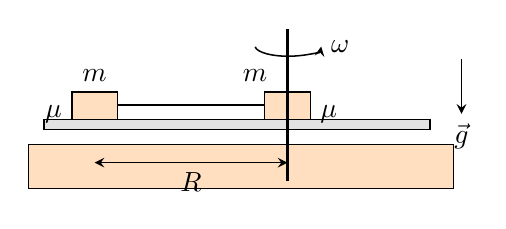
\begin{tikzpicture}[>=stealth,line width=.55pt]\draw[fill=orange!25](-.2,-.75)rectangle(5.2,-.19);\draw[fill=gray!22](0,0)rectangle(4.9,.13);\draw[fill=orange!25](.35,.13)rectangle(.93,.48) (2.8,.13)rectangle(3.38,.48);\draw[thick](3.09,-.65)--(3.09,1.28);\draw(.93,.31)--(2.8,.31);\draw[->](2.68,1.05)arc(185:357:.42 and .13)node[right]{$\omega$};\node[above]at(.64,.48){$m$};\node[above left]at(2.96,.48){$m$};\node[left]at(.35,.19){$\mu$};\node[right]at(3.38,.2){$\mu$};\draw[<->](.64,-.42)--(3.09,-.42)node[midway,below]{$R$};\draw[->](5.3,.9)--(5.3,.2)node[below]{$\vec g$};\end{tikzpicture}\end{center} На горизонтальный диск проигрывателя пластинок положили два одинаковых маленьких грузика массой m каждый, соединенных между собой горизонтальной нитью, один  — в центре, другой  — на расстоянии R  =  $12\,\text{см}$ от оси вращения (см. рисунок). Коэффициенты трения грузиков о диск одинаковы и равны $\mu=0{,}4.$ Диск начали вращать, медленно увеличивая его угловую скорость. При каком значении частоты $v$ вращения грузики свалятся с диска? Считайте, что нить невесома, нерастяжима и вначале не была натянута.
}{
\smallskip\noindent\textbf{Решение}\par
\begin{center}\begin{tikzpicture}[>=stealth,line width=.55pt]\draw[fill=orange!25](-.2,-.75)rectangle(5.2,-.19);\draw[fill=gray!22](0,0)rectangle(4.9,.13);\draw[fill=orange!25](.35,.13)rectangle(.93,.48) (2.8,.13)rectangle(3.38,.48);\draw[thick](3.09,-.65)--(3.09,1.28);\draw(.93,.31)--(2.8,.31);\draw[->](2.68,1.05)arc(185:357:.42 and .13)node[right]{$\omega$};\draw[->](.64,.31)--(.64,1.16)node[above]{$\vec N$};\draw[->](3.09,.31)--(3.09,1.16)node[above]{$\vec N$};\draw[->](.64,.31)--(.64,-.63)node[below]{$m\vec g$};\draw[->](3.09,.31)--(3.09,-.63)node[below]{$m\vec g$};\draw[->](.64,.31)--(1.61,.31)node[above]{$\vec T$};\draw[->](3.09,.31)--(2.12,.31)node[above]{$\vec T$};\draw[->](.64,.13)--(1.57,.13)node[below]{$\vec F_{\text{тр}1}$};\draw[->](3.09,.13)--(4,.13)node[above]{$\vec F_{\text{тр}2}$};\end{tikzpicture}\end{center}$1$.  Проанализируем процессы, происходящие в системе при раскручивании диска проигрывателя, изобразив силы, действующие при этом на грузики (см. рисунок). Силы натяжения, действующие на каждый груз, равны по модулю в силу невесомости нити.
$2$.  До начала раскручивания все тела находятся в покое, и сумма сил, действующих на грузики по вертикали и по горизонтали, равна нулю. Силы нормального давления N грузиков на диск и диска на грузики, одинаковые по третьему закону Ньютона, равны весам грузиков: N  =  mg. Это же соотношение выполняется и после начала раскручивания диска. 
$3$.  После начала медленного раскручивания первый грузик приобретает центростремительное ускорение $a=4 \pi ^2 \nu ^2 R,$ которое возникает по второму закону Ньютона за счет действия силы трения покоя $F_{\,\text{тр}}1 < \,\text{или} \,\text{равно} \mu N=\mu mg,$ откуда $m\omega ^2 R < \,\text{или} \,\text{равно} \mu mg.$
$4$.  В момент достижения предельного значения силы трения покоя первый грузик сдвигается и натягивает нить, то есть появляется сила натяжения нити T, действующая также и на второй грузик и возрастающая по мере ускорения вращения диска. При этом центральный грузик будет оставаться на месте, и $T=F_{\,\text{тр}}2 < \,\text{или} \,\text{равно} \mu N=\mu mg.$
$5$.  Это происходит с ростом $\omega$ до тех пор, пока сила трения $F_{\,\text{тр}}2$ не достигнет своего предельного значения $\mu mg=T_{\,\text{м}},$ после чего второй грузик начнет скользить от оси вращения, и оба грузика свалятся с диска.
$6$.  В момент начала скольжения центрального грузика по диску уравнение движения первого грузика имеет вид: $4 \pi ^2 \nu ^2 Rm=T_{\,\text{м}} + \mu mg=2\mu mg,$ откуда частота вращения диска:

\[\nu = \frac{1}{2 \pi} \sqrt{\frac{2\mu g}{R}} = \frac{1}{2 \cdot 3{,}14} \cdot \sqrt{\frac{2 \cdot 0{,}4 \cdot 10}{0{,}12}} \approx 1{,}3\,\text{Гц}.\]

Ответ: $\approx 1{,}3\,\text{Гц}.$
}

% Source 7129: https://phys-ege.sdamgia.ru/problem?id=7129
\BankTask{7129}{
\begin{center}\begin{tikzpicture}[task graph,>=stealth]\draw(4.7,0)--(0,0)--(0,2.65)--(4.7,2.65);\draw[fill=orange!35](2.5,0)rectangle(2.94,2.65);\draw[dashed](3.95,0)rectangle(4.39,2.65);\node at(1.3,1.62){\(p\)};\draw(2.82,1.02)--(3.57,1.94)node[above]{\(S\)};\draw(0,0)--(0,-.65)(2.5,0)--(2.5,-.91)(3.95,0)--(3.95,-.91);\draw[<->](0,-.49)--(2.5,-.49)node[midway,below]{\(L\)};\draw[<->](2.5,-.82)--(3.95,-.82)node[midway,below]{\(x\)};\end{tikzpicture}\end{center}
В горизонтальном цилиндрическом сосуде, закрытом поршнем, находится одноатомный идеальный газ. Первоначальное давление газа p  =  $4$ · $10^{5}$ Па. Расстояние от дна сосуда до поршня равно L. Площадь поперечного сечения поршня S  =  $25\,\text{см}^{2}$. В результате медленного нагревания газ получил количество теплоты Q  =  $1{,}65\,\text{кДж}$, а поршень сдвинулся на расстояние x  =  $10\,\text{см}$. При движении поршня на него со стороны стенок сосуда действует сила трения величиной $F_{\,\text{тр}}$  =  $3$ · $10^{3}$ Н. Найдите L. Считать, что сосуд находится в вакууме.
}{
\smallskip\noindent\textbf{Решение}\par
$1$.  Поршень будет медленно двигаться, если сила давления газа на поршень и сила трения со стороны стенок сосуда уравновесят друг друга: $p_{2}$S = $F_{\,\text{тр}}$, откуда $p_2= \frac{F_{\,\text{тр}}}{S} = 12 \cdot 10 ^{5} \,\text{Па} > p_1.$ $( p_1 = p ) .$
$2$.  Поэтому при нагревании газа поршень будет неподвижен, пока давление газа не достигнет значения $p_{2}$. В этом процессе газ получает количество теплоты $Q_{12}$. Затем поршень будет сдвигаться, увеличивая объем газа, при постоянном давлении. В этом процессе газ получает количество теплоты $Q_{23}$.
$3$.  В процессе нагревания, в соответствии с первым началом термодинамики, газ получит количество теплоты:

\[Q=Q_{12} + Q_{23} = ( U_3 - U_1 ) + p_2Sx = ( U_3 - U_1 ) + F_{\,\text{тр}}x.\]

$4$.  Внутренняя энергия одноатомного идеального газа: 

\[U_1= \frac{3}{2} \nu RT_1= \frac{3}{2} p_1SL\]

в начальном состоянии, 

\[U_3= \frac{3}{2} \nu RT_3= \frac{3}{2} p_2S ( L + x ) = \frac{3}{2} F_{\,\text{тр}} ( L + x )\]

в конечном состоянии.
$5$.  Из пп. $3$, $4$ получаем $L= \frac{Q - \frac{5}{2} F_{\,\text{тр}}x}{\frac{3}{2} ( F_{\,\text{тр}} - p_1S )} = \frac{1650 - 2{,}5 \cdot 3000 \cdot 0{,}1}{1{,}5 \cdot ( 3000 - 400000 \cdot 0{,}0025 )} =0{,}3\,\text{м}.$

Ответ: L  =  $0{,}3\,\text{м}$.
}

% Source 25727: https://phys-ege.sdamgia.ru/problem?id=25727
\BankTask{25727}{
На горизонтальном столе лежит деревянный брусок. Коэффициент трения между поверхностью стола и бруском $\mu$ = $0{,}1$. Если приложить к бруску силу, направленную вверх под углом $\alpha$ = $45$° к горизонту, то брусок будет двигаться по столу равномерно. С каким ускорением будет двигаться этот брусок по столу, если приложить к нему такую же по модулю силу, направленную под углом $\beta$ = $30^{\circ}$ к горизонту?
Какие законы Вы используете для описания движения бруска? Обоснуйте их применение к данному случаю.
}{
\smallskip\noindent\textbf{Решение}\par
Обоснование. 
$1$.  Рассмотрим задачу в системе отсчета, связанной с Землей. Будем считать эту систему отсчета инерциальной (ИСО).
$2$.  Брусок движется поступательно, поэтому описываем его моделью материальной точки. В ИСО движение материальной точки описываем вторым законом Ньютона.
$3$.  Так как брусок движется поступательно по шероховатой поверхности, то действует сила трения скольжения $F_{\,\text{тр}}=\mu N.$

Перейдем к решению. \begin{center}\begin{tikzpicture}[task graph,>=stealth]\draw(-1.8,0)--(2.2,0);\draw[fill=gray!15](-.5,0)rectangle(.5,.5);\coordinate(C)at(0,.25);\draw[dashed](0,.25)--(1.8,.25);\draw[dashed](0,1.3813708498984762)--(1.1313708498984762,1.3813708498984762)--(1.1313708498984762,.25);\draw(C)++(0:.6)arc(0:45:.6)node[midway,right]{$\alpha$};\draw(1.13137,1.38137)++(180:.4)arc(180:225:.4)node[midway,left]{$\alpha$};\draw[->,thick](C)--(1.1313708498984762,1.3813708498984762)node[above right]{$\vec F_{\text{т}}$};\draw[->,thick](C)--(0,1.9)node[above left]{$\vec N$};\draw[->,thick](C)--(0,-1)node[below]{$m\vec g$};\draw[->,thick](C)--(-1.5,.25)node[above left]{$\vec F_{\text{тр}}$};\end{tikzpicture}\end{center}
$1$.  Ускорение равно нулю, так как движение равномерное.

$\vec N + m\vec g + \vec F_{\,\text{тр}} + \vec F_{\,\text{т}} = m\vec a = 0.$

OX: $F_{\,\text{т}} \cos \alpha - \mu N = 0 \Longleftrightarrow F_{\,\text{т}} \cos \alpha = \mu N. ( 1 )$
OY: $N + F_{\,\text{т}} \sin \alpha = mg \Longleftrightarrow N= mg - F_{\,\text{т}} \sin \alpha . ( 2 )$

Из первого и второго уравнения получаем:

\[F_{\,\text{т}} \cos \alpha =\mu mg - \mu F_{\,\text{т}} \sin \alpha \Rightarrow F_{\,\text{т}}= \frac{\mu mg}{\cos \alpha + \mu \sin \alpha} . ( 3 )\]

\begin{center}\begin{tikzpicture}[task graph,>=stealth]\draw(-1.8,0)--(2.2,0);\draw[fill=gray!15](-.5,0)rectangle(.5,.5);\coordinate(C)at(0,.25);\draw[dashed](0,.25)--(1.8,.25);\draw[dashed](0,1.0499999999999998)--(1.385640646055102,1.0499999999999998)--(1.385640646055102,.25);\draw(C)++(0:.6)arc(0:30:.6);\draw(1.38564,1.05000)++(180:.4)arc(180:210:.4)node[midway,left]{$\beta$};\draw[->,thick](C)--(1.385640646055102,1.0499999999999998)node[above right]{$\vec F_{\text{т}}$};\draw[->,thick](C)--(0,1.9)node[above left]{$\vec N$};\draw[->,thick](C)--(0,-1)node[below]{$m\vec g$};\draw[->,thick](C)--(-1.5,.25)node[above left]{$\vec F_{\text{тр}}$};\end{tikzpicture}\end{center}$2$.  Ускорение не равно нулю, так как движение с ускорением.

$\vec F_{\,\text{т}} + \vec N_1 + \vec F_{\,\text{тр}1} + m\vec g = m\vec a$
OX: $F_{\,\text{т}} \cos \beta - \mu N_1 = ma \Longleftrightarrow a= \frac{F_{\,\text{т}} \cos \beta - \mu N_1}{m} . ( 4 )$
OY: $N_1 + F_{\,\text{т}} \sin \beta = mg \Longleftrightarrow N_1 = mg - F_{\,\text{т}} \sin \beta . ( 5 )$

Из четвертого и пятого уравнения получаем:

\[a= \frac{F_{\,\text{т}} \cos \beta - \mu mg + F_{\,\text{т}}\mu \sin \beta}{m} = \frac{F_{\,\text{т}} ( \cos \beta + \mu \sin \beta )}{m} - \mu g. ( 6 )\]

Из третьего и шестого уравнения получаем:

\[a= \frac{\mu mg ( \cos \beta + \mu \sin \beta )}{( \cos \alpha + \mu \sin \alpha ) m} - \mu g = \mu g ( \frac{\cos \beta + \mu \sin \beta}{\cos \alpha + \mu \sin \alpha} - 1 )\]

  — уравнение в общем виде.

\[a=0{,}1 \cdot 10 \cdot ( \frac{\cos 30 ^\circ + 0{,}1 \cdot \sin 30 ^\circ}{\cos 45 ^\circ + 0{,}1 \cdot \sin 45 ^\circ} - 1 ) \approx 0{,}18\,\text{м/с} ^2 .\]

Ответ: $0{,}18\,\text{м/с}^{2}$.
}

% Source 25952: https://phys-ege.sdamgia.ru/problem?id=25952
\BankTask{25952}{
\begin{center}\begin{tikzpicture}[task graph,>=stealth]\draw (0,0)--(3,0)--(4.8,2.5)--(1.8,2.5)--cycle (4.8,2.5)--(4.8,1.1)--(3,0);\draw (3.55,.34) arc (32:54:.65) node[midway,right]{\(\alpha\)};\draw[fill=gray!15](2.04,1.13)arc(180:360:.25 and .085)--(2.54,1.30)arc(0:180:.25 and .085)--cycle;\draw(2.04,1.30)arc(180:360:.25 and .085);\draw[->] (2.29,1.21)--(3.3,1.21) node[above]{\(\vec F\)};\end{tikzpicture}\end{center}На рисунке изображена плоскость, наклоненная под углом $\alpha =30 ^\circ$ к горизонту и тело, находящееся на ней. Если к телу приложить силу $F=1{,}7\,\text{Н},$ как показано на рисунке, то тело начнет скользить. Масса тела равна $500\,\text{г}$. Определите коэффициент трения тела о поверхность.
Какие законы Вы используете для описания движения шайбы? Обоснуйте их применение к данному случаю.
}{
\smallskip\noindent\textbf{Решение}\par
Обоснование. Систему отсчета, связанную с неподвижной плоскостью, можем считать инерциальной. Движение шайбы поступательное. Следовательно, ее можно считать материальной точкой. При движении шайбы по наклонной поверхности на него действуют силы тяжести, приложенная сила, трения и реакции опоры. В ИСО при движении тела применим второй закон Ньютона.

Перейдем к решению. На тело действуют силы:F, $F_{\,\text{тр}},$ N, $mg.$ Выберем оси координат: $\,\text{Ох}$  — вдоль нижней грани, $\,\text{О}y$  — вверх по наклонной плоскости, $\,\text{О}z$  — перпендикулярно к оси $\,\text{О}y.$ Брусок движется равномерно. Следовательно, по второму закону Ньютона: 
\begin{center}\begin{tikzpicture}[task graph,>=stealth]\draw (0,0)--(3,0)--(4.8,2.5)--(1.8,2.5)--cycle (4.8,2.5)--(4.8,1.1)--(3,0);\draw (3.55,.34) arc (32:54:.65) node[midway,right]{\(\alpha\)};\draw[fill=gray!15](2.04,1.13)arc(180:360:.25 and .085)--(2.54,1.30)arc(0:180:.25 and .085)--cycle;\draw(2.04,1.30)arc(180:360:.25 and .085);\draw[->] (2.29,1.21)--(3.3,1.21) node[above]{\(\vec F\)};\draw[->] (2.29,1.21)--(2.29,.28) node[right]{\(m\vec g\)};\draw[->] (2.29,1.21)--(1.81,2.05) node[above]{\(\vec N\)};\draw[->] (2.29,1.21)--(1.33,1.55) node[below]{\(\vec F_{\text{тр}}\)};\draw[->] (-.6,0)--(5.25,0) node[below]{\(x\)};\draw[->] (-.45,-.63)--(2.45,3.42) node[above]{\(y\)};\draw[->] (.29,-.61)--(-1.22,2.57) node[left]{\(z\)};\end{tikzpicture}\end{center}

\[\overrightarrow{F} + m\vec g + \vec N + \vec F_{\,\text{тр}}=0.\]
 
Найдем проекции на координатные оси:

\[\begin{aligned} Ox:&\quad F-F_{\text{тр},x}=0,\\Oy:&\quad F_{\text{тр},y}-mg\sin\alpha=0,\\Oz:&\quad N-mg\cos\alpha=0.\end{aligned}\]

Учитывая, что $F_{\,\text{тр}}=\mu N$ и $F_{\,\text{тр}}= \sqrt{F_{\text{тр},x}^{2}+F_{\text{тр},y}^{2}} ,$ получаем: $( \mu m g ) ^2 \cos ^2 \alpha =F ^2 + ( mg ) ^2 \sin ^2 \alpha .$

Выразим коэффициент трения:

\[\mu= \frac{\sqrt{F ^2 + ( mg \sin \alpha ) ^2}}{mg \cos \alpha} = \frac{\sqrt{1{,}7 ^2 + ( 0{,}5 \cdot 10 \cdot 0{,}5 ) ^2}}{0{,}5 \cdot 10 \cdot \cos 30 ^\circ} \approx 0{,}7.\]

Ответ: $0{,}7$.
}

% Source 43833: https://phys-ege.sdamgia.ru/problem?id=43833
\BankTask{43833}{
На горизонтальном неподвижном столе лежит доска массой $M=0{,}8\,\text{кг}$. На доске находится маленький брусок массой $m=200\,\text{г}$. Брусок и доска связаны невесомой нерастяжимой нитью, перекинутой через невесомый блок, который закреплён на стене (отрезки нити, не лежащие на блоке, горизонтальны). Коэффициент трения между бруском и доской $\mu_1=0{,}5$, между столом и доской $\mu_2=0{,}3$. Доску тянут вправо горизонтальной силой $\vec F$. Чему равен модуль силы $\vec F$, если модуль ускорения бруска относительно стола $a=1\,\text{м/с}^2$? Трением в оси блока пренебречь. Сделайте рисунок с указанием сил, действующих на тела. Обоснуйте применимость законов, используемых для решения задачи.
\begin{center}
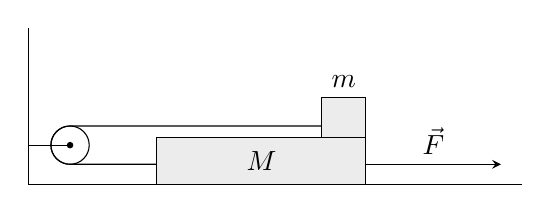
\begin{tikzpicture}[x=.64cm,y=.64cm,>=stealth]
\draw (0,3.1)--(0,0)--(9.8,0);
\draw (0,.78)--(.83,.78);
\draw (.83,.78) circle (.38);
\fill (.83,.78) circle (.065);
\draw (5.82,1.16)--(.83,1.16) arc[start angle=90,end angle=270,radius=.38]--(2.55,.40);
\draw[fill=gray!15] (2.55,0) rectangle (6.7,.94);
\draw[fill=gray!15] (5.82,.94) rectangle (6.7,1.72);
\node at (4.63,.47) {$M$};
\node[above] at (6.26,1.72) {$m$};
\draw[->] (6.7,.40)--(9.38,.40) node[midway,above] {$\vec F$};
\end{tikzpicture}
\end{center}
}{
\smallskip\noindent\textbf{Решение}\par
\textbf{Обоснование}

1. Задачу будем решать в инерциальной системе отсчёта, связанной с поверхностью стола.

2. Тела движутся поступательно, поэтому будем их описывать моделью материальной точки. Следовательно, можно использовать второй закон Ньютона, сформулированный для материальных точек. Силы, действующие на тела, постоянны, поэтому движение бруска и доски равноускоренно.

3. Так как нить нерастяжима, ускорения бруска и доски относительно стола равны по модулю и противоположны по направлению: $|\vec a_1|=|\vec a_2|=a$, $\vec a_1=-\vec a_2$. \hfill(1)

4. Так как блок и нити невесомы и трением в оси блока можно пренебречь, то силы натяжения нити, действующие на доску и брусок, одинаковы: $|\vec T_1|=|\vec T_2|=T$. \hfill(2)

5. Силы трения, действующие на брусок и доску, равны друг другу и противоположны по направлению по третьему закону Ньютона: $\vec F_{\text{тр}1}=-\vec F_{\text{тр}2}$. \hfill(3)

6. Модули сил нормальной реакции доски $\vec N_1$ и давления бруска на доску $\vec P$ также равны друг другу по третьему закону Ньютона: $N_1=P$. \hfill(4)

\textbf{Решение}

1. На рисунке показаны силы, действующие на брусок и на доску. Запишем второй закон Ньютона в проекциях на оси $Ox$ и $Oy$ выбранной системы координат. С учётом (1)–(3) получим:
\[Ma=F-F_{\text{тр}1}-F_{\text{тр}3}-T,\qquad -ma=F_{\text{тр}1}-T,\]
\[N_1=mg,\qquad N_2=Mg+P.\]

\begin{center}
\begin{tikzpicture}[x=.67cm,y=.67cm,>=stealth]
\draw[->] (0,0)--(12.05,0) node[below] {$x$};
\draw[->] (0,0)--(0,3.55) node[left] {$y$};
\node[below left] at (0,0) {$0$};
\draw (0,1.04)--(1.08,1.04);
\draw (1.08,1.04) circle (.50);
\fill (1.08,1.04) circle (.085);
\draw (7.7,1.54)--(1.08,1.54) arc[start angle=90,end angle=270,radius=.50]--(3.4,.54);
\draw[fill=gray!15] (3.4,0) rectangle (8.85,1.2);
\draw[fill=gray!15] (7.7,1.2) rectangle (8.85,2.26);
\draw[->] (8.27,1.73)--(8.27,3.23) node[right] {$\vec N_1$};
\draw[->] (8.27,1.73)--(8.27,.81) node[below right] {$m\vec g$};
\draw[->] (8.27,1.73)--(9.87,1.73) node[right] {$\vec F_{\text{тр}1}$};
\draw[->] (7.7,1.54)--(7.05,1.54) node[above] {$\vec T_1$};
\draw[->] (3.4,.54)--(2.27,.54) node[above] {$\vec T_2$};
\draw[->] (6.1,.64)--(6.1,3.02) node[left] {$\vec N_2$};
\draw[->] (6.1,.64)--(6.1,-1.38) node[right] {$M\vec g$};
\draw[->] (7.48,1.08)--(7.48,.16) node[midway,left] {$\vec P$};
\draw[->] (5.96,.92)--(4.78,.92);
\draw (4.72,1.01)--(3.92,1.60) node[above] {$\vec F_{\text{тр}2}$};
\draw[->] (5.96,.40)--(4.78,.40);
\draw (4.72,.28)--(4.15,-.34) node[below] {$\vec F_{\text{тр}3}$};
\draw[->] (8.85,.54)--(11.13,.54) node[above] {$\vec F$};
\end{tikzpicture}
\end{center}
2. Вычтя второе уравнение из первого, найдём силу, действующую на доску:
\[F=(M+m)a+2F_{\text{тр}1}+F_{\text{тр}3}.\]
3. Далее $F_{\text{тр}1}=\mu_1N_1=\mu_1mg$. С учётом (4) получим $F_{\text{тр}3}=\mu_2N_2=\mu_2(M+m)g$. В итоге:
\[\begin{aligned}F&=(M+m)(a+\mu_2g)+2\mu_1mg\\&=(0{,}8+0{,}2)(1+0{,}3\cdot10)+2\cdot0{,}5\cdot0{,}2\cdot10=6\,\text{Н}.\end{aligned}\]
Ответ: $F=6\,\text{Н}$.
}

% Source 38623: https://phys-ege.sdamgia.ru/problem?id=38623
\BankTask{38623}{
В установке, изображённой на рисунке, масса грузика $m$ подобрана так, что первоначально покоящаяся тележка после толчка вправо движется равномерно по поверхности трибометра. С каким ускорением будет двигаться тележка, если её толкнуть влево? Масса грузика $m$ в $9$ раз меньше массы тележки $M$. Блок идеален. Нить невесома и нерастяжима. Силу сопротивления движению тележки считать постоянной и одинаковой в обоих случаях. Обоснуйте применимость законов, используемых для решения задачи.
\begin{center}
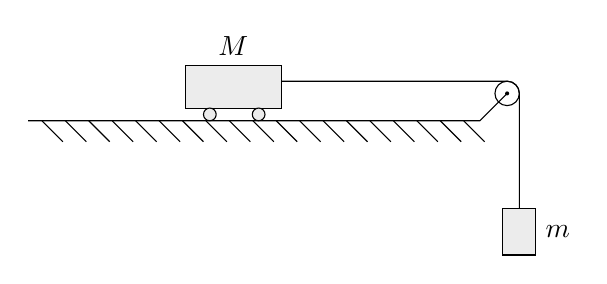
\begin{tikzpicture}[x=.62cm,y=.62cm]
\draw (0,0)--(9.25,0)--(9.81,.56);
\foreach \x in {.28,.76,...,8.96} {\draw (\x,0)--++(.43,-.43);}
\draw (9.81,.56) circle (.25);
\fill (9.81,.56) circle (.042);
\draw (5.18,.81)--(9.81,.81) arc[start angle=90,end angle=0,radius=.25]--(10.06,-1.80);
\draw[fill=gray!15] (3.22,.26) rectangle (5.18,1.13);
\draw[fill=gray!15] (3.72,.13) circle (.13);
\draw[fill=gray!15] (4.72,.13) circle (.13);
\node[above] at (4.2,1.13) {$M$};
\draw[fill=gray!15] (9.72,-1.80) rectangle (10.40,-2.75);
\node[right] at (10.40,-2.275) {$m$};
\end{tikzpicture}
\end{center}
}{
\smallskip\noindent\textbf{Решение}\par
\textbf{Обоснование.}

1. Рассмотрим задачу в системе отсчета, связанной с Землей. Будем считать эту систему отсчета инерциальной (ИСО).

2. Грузик и тележка движутся поступательно, поэтому описываем их моделью материальной точки. В ИСО движение материальной точки описываем вторым законом Ньютона.

3. Нить невесома, блок идеален (масса блока ничтожна, трения нет), поэтому модуль силы натяжения нити в любой ее точке одинаковый.

4. Нить нерастяжима, при прямолинейном поступательном движении модули ускорений грузика и тележки будут одинаковыми.

5. Движение тележки поступательное по шероховатой поверхности, поэтому на нее действует сила трения скольжения.

Перейдем к решению.

В горизонтальном направлении на тележку действуют сила трения и сила натяжения нити. В первом случае силы направлены в разные стороны и компенсируют друг друга, поэтому тележка движется равномерно. Во втором случае они обе направлены против движения, тележка движется равнозамедленно. Запишем для них второй закон Ньютона для тележки и грузика в первом случае:
\[\vec T_1+\vec F_{\text{тр}}=0,\qquad \vec T_1+m\vec g=0.\]
В проекции на оси получаем:
\[T_1-F_{\text{тр}}=0,\qquad T_1-mg=0.\]
Откуда получаем: $F_{\text{тр}}=mg$.

Запишем для них второй закон Ньютона для тележки и грузика во втором случае:
\[\vec T_2+\vec F_{\text{тр}}=M\vec a,\qquad \vec T_2+m\vec g=m\vec a.\]
В проекции на оси получаем:
\[T_2+F_{\text{тр}}=Ma,\qquad mg-T_2=ma.\]
Решая систему уравнений, имеем: $a(M+m)=F_{\text{тр}}+mg=2mg$.

В результате находим ускорение тележки:
\[a=\frac{2mg}{M+m}=\frac{2mg}{m+9m}=\frac g5=\frac{10}{5}=2\,\text{м/с}^2.\]
Ответ: $2\,\text{м/с}^2$.
}

% Source 25930: https://phys-ege.sdamgia.ru/problem?id=25930
\BankTask{25930}{
\begin{center}\begin{tikzpicture}[task graph,>=stealth]\draw (-1.4,-.4)--(3.2,-.4);\draw[fill=gray!15] (-.65,-.4) rectangle(2.45,0);\draw[double] (0,0)--(2.4,1.4);\draw (.6,0) arc (0:30:.6) node[midway,right]{\(\alpha\)};\draw(2.4,1.4)--(2.33,1.16)--(2.17,1.33)--cycle;\draw(1.6,1.42)--(3.25,1.42);\foreach \x in {1.65,1.85,...,3.05}{\draw (\x,1.42)--++(.15,.15);}\foreach \x in {-1.4,-1.2,...,3}{\draw(\x,-.4)--++(.16,-.16);}\node[above] at(.9,.65){\(m\)};\draw[->] (-.65,-.2)--(-1.85,-.2) node[above]{\(\vec F\)};\draw[->] (-.65,.8)--(-1.85,.8) node[above]{\(\vec v=\mathrm{const}\)};\end{tikzpicture}\end{center}Однородный тонкий стержень массой m = $1\,\text{кг}$ одним концом шарнирно прикреплен к потолку, а другим концом опирается на массивную горизонтальную доску, образуя с ней угол $\alpha$ = $30$°. Под действием горизонтальной силы $\vec F$ доска движется поступательно влево с постоянной скоростью (см. рис.). Стержень при этом неподвижен. Найдите F, если коэффициент трения стержня по доске \ensuremath{\mu} = $0{,}2$. Трением доски по опоре и трением в шарнире пренебречь.
Какие законы Вы используете для описания равновесия системы тел? Обоснуйте их применение к данному случаю.
}{
\smallskip\noindent\textbf{Решение}\par
Обоснование. Систему отсчета, связанную с Землей, будем считать инерциальной. Движение доски поступательное. Следовательно, ее можно принять за материальную точку. В инерциальной системе отсчета для доски, движущейся равномерно, применим второй закон Ньютона. Модуль силы трения $\vec F_{\,\text{тр}1},$ действующей на доску, равен модулю силы трения $\vec F_{\,\text{тр}2},$ действующей на стержень по третьему закону Ньютона. Кроме силы трения на стержень действуют сила реакции опоры, сила реакции шарнира, сила тяжести. Стержень будем считать абсолютно твердым телом (формы и размеры тела неизменны, расстояние между любыми двумя его точками остается неизменным). В инерциальной системе отсчета применимо правило моментов для вращающегося тела. Ось, относительно которой будем рассматривать сумму моментов сил, проведем перпендикулярно плоскости чертежа через точку крепления стержня.

Перейдем к решению.\begin{center}\begin{tikzpicture}[task graph,>=stealth]\draw[->](0,0)--(5,0)node[below]{\(x\)};\draw[->](0,0)--(0,2)node[left]{\(y\)};\node[below left]at(0,0){\(0\)};\draw[fill=gray!15](1.25,.5)rectangle(3.6,.9);\draw[->] (1.25,.7)--(.5,.7) node[above]{\(\vec F\)};\draw[->] (3.6,.7)--(4.35,.7) node[above]{\(\vec F_{\text{тр}1}\)};\end{tikzpicture}\end{center} 
$1$.  В инерциальной системе отсчета Оху, связанной с Землей, доска движется поступательно с постоянной скоростью. Поэтому сумма проекций на ось Ох всех сил, приложенных к доске, равна нулю (рис. а):

\[F_{\,\text{тр}1} - F = 0.\]

$2$.  На рис. б показаны все силы, приложенные к стержню. Силы реакции шарнира представлена горизонтальными и вертикальными составляющими: $\vec T = \vec T_1 + \vec T_2.$ По третьему закону Ньютона $\vec F_{\,\text{тр}2} = - \vec F_{\,\text{тр}1},$ поэтому

\[F_{\,\text{тр}2} = F_{\,\text{тр}1} = F. ( 1 )\]

$3$.  По условию задачи стержень покоится, поэтому сумма моментов сил относительно оси шарнира А равна нулю. Обозначив длину стержня через L, запишем это условие:\begin{center}\begin{tikzpicture}[task graph,>=stealth]\draw[double] (0,0)--(2.4,1.4);\draw (.6,0) arc (0:30:.6) node[midway,right]{\(\alpha\)};\draw[dashed](0,0)--(1.1,0);\node[above left]at(2.4,1.4){\(A\)};\draw[->] (0,0)--(0,.9) node[above]{\(\vec N\)};\draw[->] (0,0)--(-.9,0) node[below]{\(\vec F_{\text{тр}2}\)};\draw[->] (1.2,.7)--(1.2,-.78) node[right]{\(m\vec g\)};\draw[->] (2.4,1.4)--(2.4,2.4) node[above]{\(\vec T_1\)};\draw[->] (2.4,1.4)--(3.2,1.4) node[below]{\(\vec T_2\)};\end{tikzpicture}\end{center}

\[mg \frac{L}{2} \cos \alpha - F_{\,\text{тр}2}L \sin \alpha - NL \cos \alpha = 0. ( 2 )\]

$4$.  Доска движется относительно стержня, поэтому сила трения является силой трения скольжения:

\[F_{\,\text{тр}2} = \mu N. ( 3 )\]

$5$.  Подставив ($3$) в ($2$), получим уравнение

\[mg \cos \alpha - 2\mu N \sin \alpha - 2N \cos \alpha = 0,\]

позволяющее найти реакцию доски:

\[N= \frac{mg}{2 ( 1 + \mu \tan \alpha )} .\]

 Отсюда:

\[F=F_{\,\text{тр}2} = \mu N = \frac{\mu mg}{2 ( 1 + \mu \tan \alpha )} = \frac{0{,}2 \cdot 1 \cdot 10}{2 ( 1 + 0{,}2 \cdot \frac{\sqrt{3}}{3} )} \approx 0{,}9\,\text{Н}.\]

Ответ: $F \approx 0{,}9\,\text{Н}.$
}

% Source 35186: https://phys-ege.sdamgia.ru/problem?id=35186
\BankTask{35186}{
\begin{center}\begin{tikzpicture}[task graph,>=stealth]\draw(0,0)--(5,0)--(5,2)--cycle;\draw(.72,0)arc(0:21.8:.72)node[midway,right]{\(\alpha\)};\draw(1.96,1.24)circle(.42);\fill(1.96,1.24)circle(1.2pt);\draw(1.80,1.63)--(3.5,2.31);\draw(3.5,1.96)--(3.5,2.69);\foreach \y in {2,2.12,...,2.66}{\draw(3.5,\y)--++(.14,-.12);}\draw(1.96,1.24)--(2.38,1.24)node[right]{\(R\)};\end{tikzpicture}\end{center} На шероховатой наклонной плоскости покоится цилиндр. К верхней части цилиндра по касательной прикреплена параллельная наклонной плоскости невесомая нерастяжимая нить, другой конец которой закреплен на вертикальной стене. Масса цилиндра $1\,\text{кг}$, радиус его основания $20\,\text{см}$, коэффициент трения цилиндра о наклонную плоскость $0{,}5$. Определить предельный угол альфа, при котором цилиндр будет находиться в равновесии. Какие законы Вы используете для решения задачи? Обоснуйте их применение.
}{
\smallskip\noindent\textbf{Решение}\par
\begin{center}\begin{tikzpicture}[task graph,>=stealth]\draw(0,0)--(5,0)--(5,2)--cycle;\draw(.72,0)arc(0:21.8:.72)node[midway,right]{\(\alpha\)};\draw(1.96,1.24)circle(.42);\fill(1.96,1.24)circle(1.2pt);\draw(1.80,1.63)--(3.5,2.31);\begin{scope}[shift={(3.7,2.39)},rotate=21.8]\draw[fill=gray!15](-.22,-.22)rectangle(.22,.22);\end{scope}\node[below right]at(2.12,.85){\(A\)};\draw[->] (1.96,1.24)--(1.20,2.17) node[left]{\(\vec N\)};\draw[->] (1.80,1.63)--(3.02,2.12) node[above]{\(\vec T\)};\draw[->] (2.12,.85)--(3.29,1.32) node[below]{\(\vec F_{\text{тр}}\)};\draw[->] (1.96,1.24)--(1.96,.15) node[right]{\(m\vec g\)};\end{tikzpicture}\end{center}Обоснование. $1$.  Рассмотрим задачу в системе отсчета, связанной с Землей. Будем считать эту систему отсчета инерциальной (ИСО).
$2$.  Описываем цилиндр моделью твердого тела (форма и размеры тела неизменны, расстояние между двумя точками тела остается неизменным ).
$3$.  Любое движение твердого тела является суперпозицией поступательного и вращательного движений. Поэтому условий равновесия твердого тела в ИСО ровно два: одно −для поступательного движения, другое − для вращательного движения.
$4$.  В качестве оси, относительно которой будем считать сумму моментов сил, действующих на цилиндр, выберем ось, проходящую перпендикулярно плоскости рисунка через точку касания цилиндра плоскости А.
$5$.  Нить невесома, поэтому модуль силы натяжения нити в любой ее точке один и тот же.
$6$.  Между цилиндром и поверхностью наклонной плоскости действует сила трения, которая в предельном случае равна $F_{\,\text{тр}}=\mu N.$
Перейдем к решению. Изобразим все силы, действующие на цилиндр: сила тяжести mg, сила реакции опоры N, сила трения F$_{\,\text{тр}}$, сила натяжения нити Т.
Запишем правило моментов относительно точки А:

\[mg \sin \alpha \cdot R - T \cdot 2R=0.\]

Тогда получаем, что $T= \frac{mg \sin \alpha}{2} .$
Применим второй закон Ньютона, учитывая, что ускорение равно $0$:

\[\vec N + \vec T + m\vec g + \vec F_{\,\text{тр}}=0.\]

Найдем проекцию на оси:

$Ox:T + F_{\,\text{тр}} - mg \sin \alpha =0;$
$Oy:N - mg \cos \alpha =0.$

Учитывая, что в предельном случае сила трения равна $F_{\,\text{тр}}=\mu N,$ получаем:

\[T + \mu mg \cos \alpha - mg \sin \alpha =0.\]

Объединяя уравнения, получаем:

\[2\mu \cos \alpha = \sin \alpha .\]

Откуда находим предельный угол наклона плоскости

\[\alpha = \arctan 2\mu= \arctan ( 2 \cdot 0{,}5 ) =45 ^\circ .\]

Данный угол действительно будет максимальным, поскольку при увеличении угла наклона сила трения уменьшится, горизонтальная составляющая силы тяжести увеличится, сила натяжения нити увеличится, в результате чего равновесие нарушится.

Ответ: $45$°.
}

\end{document}
